\newpage
\section{Eingabe}
    \subsection{Tastenbyte auslesen}
        Um auf einen Tastendruck zu reagieren wird in regelmäßigen Abstand das \textit{PIO\_B}-Byte ausgelesen.
        Dabei ist dieses \textit{n-aus-8-Kodiert}. Jedes Bit repräsentiert dabei den Zustand eines Tasters.
        Ist ein Bit auf 0 gesetzt, ist die Taste zurzeit gedrückt und umgekehrt.

        \begin{description}
            \item [Taste 0 (11111110)]
            Setzt abhängig davon wer zurzeit dran ist, einen entsprechenden Stein an der Cursorposition.
            Sobald der Stein gesetzt worden ist, wird die Logik angesteuert um einen möglichen Sieg zu ermitteln.
            \item [Taste 1 (11111101)] Bewegt den Cursor nach Links.
            \item [Taste 3 (11110111)] Bewegt den Cursor nach Rechts.
            \item [Taste 4 (11101111)] Setzt das Spiel zurück.
        \end{description}


    \subsection{Flankenerkennung und Entprellung}
        Da das einlesen des \textit{PIO\_B}-Bytes in einer Schleife **SIEHE MAINLOOP** ausgeführt wird,
        muss sichergestellt werden, dass nur eine Flanke pro Tastendruck ausgewertet wird.
        Zusätzlich muss, durch die fehlende Hardwareentprellung der Tasten, die Entprellung in Software realisiert werden.
        \\
        \\
        Dazu wird zunächst das \textit{buttonFlag} getestet. Ist es nicht gesetzt, kann auf eine Taste reagiert und
        das Flag gesetzt werden. Ist es jedoch gesetzt, wird ein Timer inkrementiert.
        Ist dieser größer als 250, wird das \textit{buttonFlag} zurück gesetzt,
        welches es wieder ermöglicht auf einen Tastendruck zu reagieren.
        Falls der Timer jedoch kleiner als 250 ist, muss weiterhin gewartet werden umd ein Entprellen der Tasten
        zu gewährleisten.

        \begin{figure}[H]
            \centering
            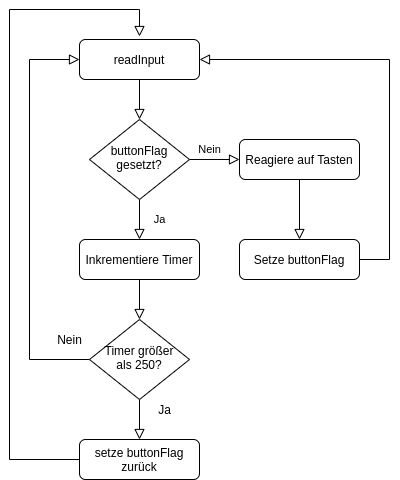
\includegraphics[scale=0.5]{img/entprellung.png}    
            \caption{Programmablaufplan: \textit{readInput}}
        \end{figure}
